\documentclass[titlepage,11pt]{article}
\usepackage{comment}
\usepackage{enumitem}
\usepackage{transparent} % Untuk transparansi gambar
\usepackage{listings}
\usepackage{amsmath}
\usepackage{graphicx}
\usepackage[font=small,labelfont=bf]{caption}
\usepackage[bahasa]{babel}
\usepackage{float}
\usepackage{verbatim}
\usepackage{graphicx,tabularx,multirow}
\usepackage{xcolor}
\usepackage[onehalfspacing]{setspace}
\usepackage[
	allcolors=visigrey,
	colorlinks=true,
]{hyperref}
\usepackage[a4paper,left=2cm,right=2cm]{geometry}
% Pengaturan kutipan artikel
\usepackage[style=ieee, backend=biber]{biblatex}
%Code listing style pak akok
\definecolor{codegreen}{rgb}{0,0.6,0}
\definecolor{codegray}{rgb}{0.5,0.5,0.5}
\definecolor{codepurple}{rgb}{0.58,0,0.82}
\definecolor{backcolour}{rgb}{0.95,0.95,0.92}

\usepackage{eso-pic} % Untuk menambahkan elemen ke seluruh halaman

\newcommand\BackgroundPic{
  \put(0,0){
    \parbox[b][\paperheight]{\paperwidth}{
      \vfill
      \centering
      \transparent{0.1}
      \includegraphics[width=0.4\paperwidth,keepaspectratio]{miot.png}
      \vfill
    }
  }
}

\newcommand\BackgroundAllPages{ \AddToShipoutPicture*{\BackgroundPic} }
\newcommand\BackgroundNone{ \ClearShipoutPicture } % hilangkan background

\lstdefinestyle{mystyle}{
	backgroundcolor=\color{backcolour}, commentstyle=\color{codegreen},
	keywordstyle=\color{magenta},
	numberstyle=\small\color{codegray},
	stringstyle=\color{codepurple},
	basicstyle=\ttfamily\footnotesize,
	breakatwhitespace=false,         
	breaklines=true,                 
	captionpos=t,                    
	keepspaces=true,                 
	numbers=left,                    
	numbersep=5pt,                  
	showspaces=false,                
	showstringspaces=false,
	showtabs=false,           
	frame = single,
	tabsize=2
}
\lstset{style=mystyle}

\definecolor{visigrey}{rgb}{.1,.15,.15}
\geometry{top=1cm,bottom=.5cm}
\savegeometry{titlepage}
\geometry{top=2cm,bottom=2cm}
\savegeometry{main}

\def\bspace{\(\qquad\qquad\qquad\)}
\usepackage[T1]{fontenc}
\usepackage[utf8]{inputenc}
\usepackage{tgheros}
\renewcommand*\familydefault{\sfdefault}

\setcounter{tocdepth}{6}

\def\autor{Laboratorium }
\def\lab{Multimedia dan Internet of Things}
\def\departemen{Departemen Teknik Komputer}
\def\institut{Institut Teknologi Sepuluh Nopember}
\def\praktikum{Laporan Akhir \\ Praktikum Jaringan Komputer}
\def\nama{Muhammad Ibnu - 5024231123}
% Ubah Judul sesuai dengan modul
\def\judul{Crimping dan Routing IPv4}
\def\tanggal{2025}
\begin{document}
% Ubah Bahasa sesuai dengan keinginan
\selectlanguage{bahasa}

\BackgroundNone
\def\headingtype{\bf \small}
\loadgeometry{titlepage}

\begin{titlepage}
	\centering
	\begin{tabularx}{\textwidth}{l@{\hskip 0pt}lX}
		\raisebox{-0.5\height}{
\includegraphics[width=3cm]{Cover/img/logodepart.png}} 
		& \raisebox{-0.5\height}{\includegraphics[width=3cm]{Cover/img/miot.png}} 
		& \raggedleft
	\hfill
	\begin{minipage}{0.5\textwidth}
		\raggedleft
		{\emph{\headingtype \autor}} \\[-2pt]
		{\headingtype \lab} \\[-2pt]
		{\headingtype \departemen} \\[-2pt]
		{\headingtype \emph{\institut}}
	\end{minipage}

	\vspace{5cm}
	\end{tabularx}
	
	\vspace{5cm}
	{\Huge \bf \praktikum \par}
	
	\vspace{2cm}
	{\LARGE \bf \judul \par}
	
	\vspace{2cm}
	{\Large \nama \par}
	
	\vfill
	{\Large \tanggal \par}
	
	\vfill
	
\includegraphics[width=\textwidth]{Cover/img/footer.png}
\end{titlepage}

\loadgeometry{main}


\BackgroundAllPages
% Pilih Modul yang akan di build
\section{Pendahuluan}
\subsection{Latar Belakang}
Dalam era digital saat ini, jaringan komputer merupakan infrastruktur utama yang mendukung komunikasi data, baik di lingkungan rumah, kantor, hingga pusat data skala besar. Agar jaringan dapat berfungsi secara optimal, pemahaman tentang aspek fisik dan logis dari jaringan sangat penting. Dua aspek mendasar yang menjadi fokus dalam praktikum ini adalah crimping kabel jaringan dan routing IPv4. Crimping merupakan proses pembuatan kabel jaringan dengan konektor RJ-45 yang sesuai standar, seperti straight-through dan crossover. Proses ini penting karena koneksi fisik yang buruk dapat menyebabkan gangguan komunikasi jaringan. Dengan memahami dan mempraktikkan teknik crimping, mahasiswa dapat memastikan kualitas koneksi jaringan yang andal dan efisien, sekaligus mengenal perbedaan penggunaan kabel berdasarkan jenis perangkat yang dihubungkan.Di sisi lain, routing IPv4 merupakan proses pengaturan jalur pengiriman data antar jaringan menggunakan alamat IP versi 4. Dalam praktiknya, routing memungkinkan komputer di jaringan berbeda untuk saling terhubung melalui perangkat router. Pemahaman tentang routing sangat krusial, terutama dalam membangun jaringan skala menengah hingga besar yang terdiri atas banyak subnet dan perangkat. Menguasai konsep ini juga relevan dengan implementasi di dunia nyata, seperti konfigurasi jaringan kantor, ISP, dan sistem komunikasi antar-cabang perusahaan. Dengan demikian, praktikum ini bertujuan untuk memberikan pemahaman menyeluruh mulai dari pembuatan koneksi fisik jaringan hingga pengaturan logika pengiriman data. Melalui kegiatan ini, mahasiswa diharapkan mampu mengatasi masalah dasar dalam jaringan serta memahami pentingnya keterampilan jaringan komputer dalam menunjang berbagai teknologi modern seperti cloud computing, IoT, dan layanan berbasis internet lainnya.

\subsection{Dasar Teori}
Crimping adalah proses penghubungan kabel jaringan dengan konektor RJ-45 menggunakan alat crimping untuk memastikan sambungan yang kuat dan stabil antara kabel dan perangkat jaringan. Proses ini melibatkan penggunaan kabel UTP (Unshielded Twisted Pair) yang terdiri dari pasangan kawat yang dipilin untuk mengurangi gangguan elektromagnetik. Kabel ini memiliki dua jenis konfigurasi utama, yaitu kabel straight-through yang digunakan untuk menghubungkan perangkat yang berbeda, seperti PC ke switch atau router, dan kabel crossover yang digunakan untuk menghubungkan perangkat yang sama, seperti switch ke switch atau PC ke PC. Konektor RJ-45 terdiri dari 8 pin yang terhubung dengan kawat di dalam kabel UTP, dan dalam crimping, urutan kabel yang benar sangat penting untuk memastikan transmisi data yang stabil dan aman. Routing IPv4 merupakan proses pengaturan jalur pengiriman data antar jaringan menggunakan alamat IP versi 4, yang terdiri dari alamat sepanjang 32-bit yang dibagi menjadi 4 dan dipisahkan oleh titik. Alamat ini dapat dikelompokkan dalam berbagai subnet untuk membagi jaringan menjadi segmen-segmen yang lebih kecil. Router berfungsi untuk menentukan jalur pengiriman data melalui jaringan berdasarkan informasi yang terdapat dalam tabel routing, yang berisi alamat tujuan, netmask, dan gateway. Routing dapat dilakukan secara statis, di mana administrator jaringan menentukan jalur secara manual, atau dinamis, dengan menggunakan protokol routing otomatis seperti RIP, OSPF, dan EIGRP. Subnetting adalah proses membagi alamat IP menjadi beberapa subnet untuk mengoptimalkan penggunaan alamat IP, memungkinkan pengelolaan jaringan yang lebih efisien. Konsep crimping dan routing ini merupakan bagian penting untuk menciptakan jaringan yang andal, di mana crimping memastikan koneksi fisik yang optimal dan routing mengelola pengiriman data antar jaringan. Pemahaman tentang kedua konsep ini pun sangat penting dalam membangun dan mengelola jaringan komputer yang efisien dan efektif.


%===========================================================%
\section{Tugas Pendahuluan}
Bagian ini berisi jawaban dari tugas pendahuluan yang telah anda kerjakan, beserta penjelasan dari jawaban tersebut
\begin{enumerate}
	\item 
	\begin{enumerate}
		\item Rentang IP address dan prefix (CIDR) yang sesuai untuk masing-masing departemen.\\
		Setiap departemen memiliki kebutuhan perangkat dan konektivitas yang berbeda-beda. Dalam menetukan besar subnet atau untuk setiap departemen, selain mempertimbangkan jumlah perangkat yang terhubung, juga harus memperhatikan kebutuhan tambahan 2 alamat untuk network address dan broadcast. Berdasarkan kebutuhan address ini, kemudian ditentukan ukuran subnetnya dengan mencari perpangkatan 2 yang paling mendekati dan lebih besar dari kebutuhan. Misal pada departemen produksi memerlukan 52 address, perpangkatan 2 yang paling mendekati adalah $2^6$ atau 64. Sehingga, prefix yang dipakai untuk subnet departemen ini adalah /26 yang diambil dari ukuran network portion yang tersisa dikurangkan dengan host portion yang digunakan atau $32-6$. Prefix untuk departemen lain tercantum dalam tabel \ref{tab:tupen1a}. Dalam menetukan rentang alamat, digunakan alamat ipv4 dari kelas C dengan memulai alokasi dari subnet dengan prefix terkecil, yaitu RnD. Alokasi rentang address juga dapat dilihat pada tabel \ref{tab:tupen1a}.
			\begin{longtable}{|c|c|>{\centering\arraybackslash}m{2cm}|>{\centering\arraybackslash}m{1.5cm}|c|>{\centering\arraybackslash}m{3cm}|}
				\caption{Rentang IP address dan Prefix (CIDR)}
				\label{tab:tupen1a} \\
				\hline
				No & Departemen & Jumlah \, Perangkat & Jumlah Minimal \, Address & Prefix & Rentang Address \\ 
				\hline
				\endfirsthead
				\hline
				No & Departemen & Jumlah Perangkat & Jumlah Minimal Address & Prefix & Rentang Address \\ 
				\hline
				\endhead
				\hline
				\endfoot
				\hline
				\endlastfoot
				1 & Produksi & 50 & 52 & /26 & 192.168.0.128 \, - \, 192.168.0.191 \\ \hline
				2 & Administrasi & 20 & 22 & /27 & 192.168.0.192 \, - \, 192.168.0.223\\ \hline
				3 & Keuangan & 10 & 12 & /28 & 192.168.0.224 \, - \, 192.168.0.239 \\ \hline
				4 & RnD & 100 & 102 & /25 & 192.168.0.0 \, - \, 192.168.0.127
			\end{longtable}
		\item Total subnet yang diperlukan dan IP network untuk masing-masing. \\
		Di perusahaan ini, hanya menggunakan 1 router dan jaringan dibagi ke 4 departemen, maka jumlah subnet yang diperlukan adalah 4. Pembagian IP Network untuk masing-masing departmen tersaji dalam tabel \ref{tab:tupen1b}.
		\begin{longtable}{|c|c|c|>{\centering\arraybackslash}m{3cm}|c|}
			\caption{Pembagian Network Address} \label{tab:tupen1b} \\
			\hline
			No & Departemen & Network Address & Usable \, IP Address & Broadcast Address \\
			\hline
			\endfirsthead
			\hline
			No & Departemen & Network Address & Usable \, IP Address & Broadcast Address \\
			\hline
			\endhead
			\hline
			\endfoot
			\hline
			\endlastfoot
				1 & Produksi & 192.168.0.128 & 192.168.0.129 \, - \, 192.168.0.190 & 192.168.0.191 \\ \hline
				2 & Administrasi & 192.168.0.192 & 192.168.0.193 \, - \, 192.168.0.222 & 192.168.0.223 \\ \hline
				3 & Keuangan & 192.168.0.224 & 192.168.0.225 \, - \, 192.168.0.238 & 192.168.0.239 \\ \hline
				4 & RnD & 192.168.0.0 & 192.168.0.1 \, - \, 192.168.0.126 & 192.168.0.127 \\ \hline
			\end{longtable}
	\end{enumerate}
	\item Topologi Network 
	\begin{figure}[!h] 
    \centering
    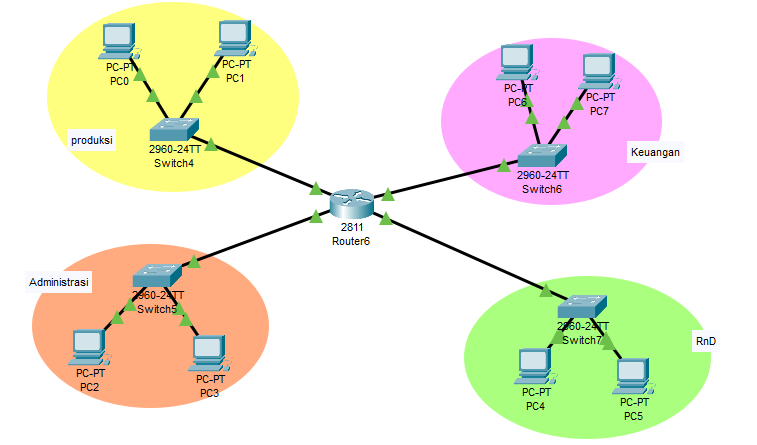
\includegraphics[width=0.5\textwidth]{P1/img/tupen2.png}
    \caption{Topologi Network Perusahaan}
    \label{fig:Topologi Network Perusahaan}
	\end{figure}
	\item Table Routing\\
	Dalam soal, hanya menggunakan 1 router, sehingga tidak memerlukan skema routing apapun. Jika menggunakan skema routing, maka diperlukan setidaknya 2 router. Oleh karena itu, perlu pencocokan menjadi seperti pada gambar \ref{fig:Topologi Network Perusahaan dengan 2 Router} dengan tambahan 1 subnet 192.168.0.240/29. Router 1 (192.168.0.242) terhubung ke departemen Administrasi dan Produksi sedangkan router 2 (192.168.0.241) terhubung ke departemen RnD dan Keuangan
	\begin{figure}[!h] 
    \centering
    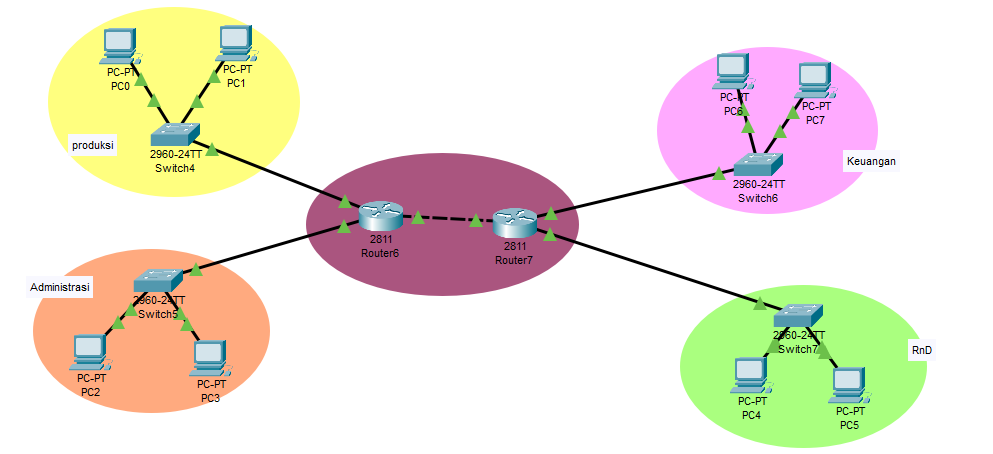
\includegraphics[width=0.5\textwidth]{P1/img/tupen3.png}
    \caption{Topologi Network Perusahaan dengan 2 Router}
    \label{fig:Topologi Network Perusahaan dengan 2 Router}
	\end{figure}
	\begin{longtable}{|c|c|c|c|}
		\caption{Table Routing Router 1}
		\label{tab:tupen4} \\
		\hline
		Network Destination & Netmask/Prefix & Gateway & Interface Tujuan \\
		\hline
		\endfirsthead
		\hline
		Network Destination & Netmask/Prefix & Gateway & Interface Tujuan \\
		\hline
		\endhead
		\hline
		\endfoot
		\hline
		\endlastfoot
		192.168.0.0 & 255.255.255.128/25 & 192.168.0.3 & 192.168.0.241 \\ \hline
		192.168.0.128 & 255.255.255.192/26 & 192.168.0.31 & 192.168.0.242 \\ \hline
		192.168.0.192 & 255.255.255.224/27 & 192.168.0.195 & 192.168.0.242 \\ \hline
		192.168.0.224 & 255.255.255.240/28 & 192.168.0.117 & 192.168.0.241 \\ \hline
		\end{longtable}
	\item Berdasarkan topologi yang telah dibuat, skema routing yang paling cocok untuk perusahaan baru ini adalah \emph{Static Routing}. Terdapat beberapa alasan kenapa skema ini lebih cocok. Pertama topologi sederhana. Hanya ada 2 router, dan masing-masing router hanya perlu tahu jalur ke 2 subnet tambahan yang tidak langsung terhubung dengannya. Ini bisa dengan mudah dikonfigurasi secara manual menggunakan static route. Kedua, jalur antar router tetap. Karena hanya ada satu jalur tetap antara Router 1 dan Router 2, tidak ada kebutuhan untuk dinamika perhitungan jalur seperti dalam routing dinamis. Ketiga, lebih ringan dan efisien untuk kasus perusahaan baru ini. Untuk kebutuhan topologi network kecil to medium, skema static router lebih efisien daripada skema lainnya.
\end{enumerate}

\end{document}